\documentclass{cumcm}
\usepackage{graphicx}
\usepackage{appendix}
\numberwithin{equation}{section}
\numberwithin{equation}{subsection}
\usepackage{csvsimple}
\usepackage{listings}
\usepackage{xcolor}
%\renewcommand{\baselinestretch}{1.0}
%\newcommand{\songtiB}

% \title{text}这里是显示在第三页的文章标题
\title{\textbf{计算机系统结构实验报告\quad 实验6}\\{\Large 类MIPS多周期流水线处理器的设计与实现}}
\author{方泓杰\ 518030910150}


\begin{document}
\maketitle

\begin{abstract}
  本实验实现了类MIPS多周期流水线处理器的几个重要部件,该类MIPS多周期流水线处理器的CPU支持全部31条MIPS指令。本实验以实验三、四实现的模块以及实验五实现的类MIPS单周期处理器为基础,对部分功能进行了修改,添加了部分控制信号;同时,为适应流水线结构,增加了段寄存器,支持通过前向通路(forwarding)与流水线停顿(stall)来解决流水线冒险;同时通过预测不转移(predict-not-taken)策略解决控制竞争问题所带来的高延迟,提高流水线性能。本实验通过软硬法仿真的形式进行实验结果的验证。
\end{abstract}

\maketitle \tableofcontents
\newpage

\section{实验目的}\label{section1}
本次实验有如下六个实验目的:
\begin{enumerate}
    \item 理解CPU Pipeline,了解流水线冒险(hazard)及相关性,设计基础流水线CPU;
    \item 设计支持Stall的流水线CPU。通过检测竞争并插入停顿(Stall)机制解决数据冒险、控制竞争和结构冒险;
    \item 在2的基础上,增加Forwarding机制解决数据竞争,减少因数据竞争带来的流水线停顿延时,提高流水线处理器性能(也允许将Stall与Forwarding结合实现);
    \item 在3的基础上,通过predict-not-taken或延时转移策略解决控制冒险/竞争,减少控制竞争带来的流水线停顿延时,进一步提高处理器性能(也允许将2、3、4结合实现);
    \item 在4的基础上,将CPU支持的指令数量从16条扩充到31条,使处理器性能更加丰富(选做);
    \item 使用功能仿真验证功能实现的正确性。
\end{enumerate}

\section{原理分析}\label{section2}

\subsection{各模块原理分析}\label{section2.1}

\subsubsection{主控制器(Ctr)、运算单元控制器(ALUCtr)原理分析}\label{section2.1.1}
主控制器需要对指令的最高6位的OpCode域进行解析,初步判断指令的类型并产生对应的处理器控制信号。我们在主控制器中\underline{对除jr外的其余R型指令不作区分},留给运算单元控制器(ALUCtr)做进一步的区分;其余指令均作区分。本次实验中用到的控制信号如表 \ref{tab1} 所示。

\begin{table}[htbp]
    \centering
    \begin{tabular}{|c|c|}
         \hline
         信号 & 具体说明 \\ \hline
         ALUSrc & 算术逻辑运算单元(ALU)的第二个操作数的来源(0:使用rt;1:使用立即数)\\
         ALUOp (*) & 发送给运算单元控制器(ALUCtr)用来进一步解析运算类型的控制信号 \\
         beqSign & 条件跳转beq指令信号,高电平说明当前指令是beq指令 \\
         bneSign & 条件跳转bne指令信号,高电平说明当前指令时bne指令 \\
         extSign & 符号扩展信号,高电平说明当前指令需要进行符号拓展 \\
         jalSign & jal指令信号,高电平说明当前指令是jal指令 \\
         jrSign & jr指令信号,高电平说明当前指令是jr指令 \\
         luiSign & lui指令信号,高电平说明当前指令是lui指令 \\
         Jump & 无条件跳转信号,高电平说明当前指令是无条件跳转指令(j或jal,此处不含jr) \\
         memRead & 内存读使能信号,高电平说明当前指令需要进行内存读取(load) \\
         memToReg & 写寄存器的数据来源 (0:使用ALU运算结果;1:使用内存读取数据) \\
         memWrite & 内存写使能信号,高电平说明当前指令需要进行内存写入(store) \\
         regDst & 目标寄存器的选择信号(0:写入rt代表的寄存器;1:写入rd代表的寄存器)\\
         regWrite & 寄存器写使能信号,高电平说明当前指令需要进行寄存器写入 \\
         \hline
    \end{tabular}
    \caption{主控制器产生的控制信号}
    \label{tab1}
\end{table}

上表中标(*)的ALUOp信号包含四个二进制位。我们重新将ALUOp与ALUCtr进行\underline{联合设计},也就是说,ALUOp将可以解析的指令的ALUCtrOut控制信号都解析完成,其余不能确定具体类型的R型指令留给运算单元控制器(ALUCtr)做进一步的解析,已经解析完成的指令的ALUOp直接可以称为运算单元控制器中ALUCtrOut的输出。

\begin{table}[htbp]
    \centering
    \begin{tabular}{|c|c|c|}
         \hline
         ALUOp / ALUCtrOut 的信号内容 & 指令 & 具体说明 \\
         \hline
         0000 & add, addi & ALU执行带溢出检查的加法 \\
         0001 & addu, addiu, lw, sw & ALU执行不带溢出检查的加法 \\
         0010 & sub, subi & ALU执行带溢出检查的减法 \\
         0011 & subu, beq, bne & ALU执行不带溢出检查的减法 \\
         0100 & and, andi & ALU执行逻辑与运算 \\
         0101 & or, ori & ALU执行逻辑或运算 \\
         0110 & xor, xori & ALU执行逻辑异或运算 \\
         0111 & nor & ALU执行逻辑或非运算 \\
         1000 & slt, slti & ALU执行带符号小于时置位运算 \\
         1001 & sltu, sltiu & ALU执行无符号小于时置位运算 \\
         1010 & sll, sllv, lui & ALU执行逻辑左移运算 \\
         1011 & srl, srlv & ALU执行逻辑右移运算 \\
         1100 & sra, srav & ALU执行算术右移运算 \\
         1101 / 1110 & 无 & 未定义 \\
         1111 & j, jal, jr & ALU不进行任何操作 \\
         \hline
    \end{tabular}
    \caption{ALUOp信号的具体含义以及解析方式}
    \label{tab2}
\end{table}

经过联合设计,假如我们令在主控制器中未解析出来的指令的ALUOp为1101(未定义),那么在运算单元控制器(ALUCtr)中,我们只要对未定义的ALUOp值进行进一步解析即可,其余指令可以沿用ALUOp作为ALUCtrOut输出;这样设计更加方便。

同时注意到,我们增添了一些新的控制信号;因篇幅所限,这里不再列出主控制器(Ctr)产生的各种控制信号与指令OpCode域的对应方式;可以参照指令的含义以及表 \ref{tab1} 所示的信号含义进行解析,方法与实验三时所用的方法相同。当出现其他暂不支持的指令时,我们将所有的控制信号均置为0,将这条指令看作一条空指令(nop),使得该指令对数据没有影响,保证数据的正确性。

与实验五类似,我们在运算单元控制器(ALUCtr)中增加两个信号jrSign与shamtSign,分别用来表示该指令是否为jr、该指令操作数是否在shamt中。这两个信号将会在指令解析完成后进行处理。

\subsubsection{算术逻辑运算单元(ALU)原理分析}\label{section2.1.2}

ALU主要根据由运算单元控制器(ALUCtr)产生的运算单元控制信号ALUCtrOut,对输入的两个数执行对应的算术逻辑运算,输出运算的结果以及部分控制信号。其输出的一个重要信号为 zero 信号,当运算结果为 0 时该信号为高电平,否则为低电平;该信号用于与 branch 指令结合判断是否满足转移条件。ALU执行的算术逻辑运算类型与运算单元控制信号ALUCtrOut的对应方式在第 \ref{section2.1.1} 节中已提及,可以参见第 \ref{section2.1.1} 节中的表 \ref{tab2}。

\subsubsection{寄存器(Register)原理分析}\label{section2.1.3}

本部分和实验四的寄存器的原理分析基本相同。唯一的一个区别是,我们增加了对于jal指令的支持,由于jal默认将下一条指令的地址保存至寄存器31,于是我们在寄存器文件上增加了一个新的接口用于处理jal指令带来的特殊情况。其余部分和实验四的寄存器完全相同。

\subsubsection{存储器(Data Memory)原理分析}\label{section2.1.4}

本部分和实验四的存储器的原理分析完全相同,不再赘述。

\subsubsection{指令存储器(Instruction Memory)原理分析}\label{section2.1.5}

本部分和第 \ref{section2.1.4} 节中的存储器几乎相同,而且不需要支持修改操作。因此在读入初始数据后,后续只要直接输出给定的输入PC值所指向的指令即可。

\subsubsection{有符号扩展单元(Sign Extension)原理分析}\label{section2.1.6}

本部分和实验四的有符号扩展单元的原理分析完全相同,不再赘述。

\subsubsection{数据选择器(Mux)原理分析}\label{section2.1.7}

本部分和实验五的数据选择器的原理分析完全相同,不再赘述。

\subsubsection{程序计数器模块(PC)原理分析}\label{section2.1.8}

在本次实验中,我们不再设置单独的PC模块,而是利用阻塞赋值完成延迟到时钟上升沿赋值的操作;所以在本次实验中,我们将这个模块简化为顶层模块中的一个全局寄存器PC。

\subsection{流水线各阶段原理分析}\label{section2.2}

\subsubsection{取指阶段(Instruction Fetch, IF)}\label{section2.2.1}

取指阶段主要包含程序计数器模块(PC)以及指令存储器(Instruction Memory)模块,主要原理是根据程序计数器模块提供的PC从指令存储器中取出当前指令。

\subsubsection{译码阶段(Instruction Decode, ID)}\label{section2.2.2}

译码阶段主要包含主控制器模块(Ctr)、寄存器模块(Registers)以及有符号扩展单元(Sign Extension),还包含一个利用regDst控制信号对运算结果在rt与rd之间进行选择的选择器(虽然这个信号在最后一个周期才真正用到,但是为减少传输不必要数据与段寄存器的空间开销,我们提前处理该信号),主要原理是根据指令译码得到各控制信号,同时进行有符号拓展与运算结果寄存器的选择。

\subsubsection{执行阶段(Execution, EX)} \label{section2.2.3}
执行阶段主要包括运算单元控制器(ALUCtr)、算术逻辑运算单元(ALU)以及一系列对于运算数的选择器(如利用shamtSign控制信号对运算数1在rs与shamt中选择的选择器、利用ALUSrc控制信号在对运算数2在rt与有符号扩展结果中选择的选择器等等),主要原理是对部分指令继续进行指令的更加细致的译码,同时算数逻辑运算单元执行指令中对应的运算。

\subsubsection{访存阶段(Memory Access, MA)}\label{section2.2.4}
访存阶段主要包括存储器(Data Memory)以及一个利用memToReg信号对结果在ALU运算结果以及访存结果中选择的选择器,主要原理是进行内存的访问(读/写)。

\subsubsection{写回阶段(Write Back, WB)}\label{section2.2.5}
写回阶段主要包括对寄存器的写回,我们将写回安排在时钟下降沿进行操作,这样可以有效解决一部分的数据冒险。

\subsection{顶层模块(Top)原理分析}\label{section2.3}

\subsubsection{流水线段寄存器}\label{section2.3.1}

在流水线的两个阶段之间,我们需要设置一系列的段寄存器,用于保存指令在上一阶段执行的结果,我们将所用到的段寄存器以及其中存储的内容列出如下:

\begin{itemize}
    \item \textbf{IF $\rightarrow$ ID 段寄存器}:主要包含当前指令及其PC;
    \item \textbf{ID $\rightarrow$ EX 段寄存器}:主要包含控制信号(包括ALUOp、ALUSrc、luiSign、beqSign、bneSign、memWrite、memRead、memToReg、regWrite信号)、有符号扩展单元的结果、解析出的指令rs、rt、funct、shamt的值、读rs与rt寄存器得到的结果、当前指令PC与目标寄存器的地址;
    \item \textbf{EX $\rightarrow$ MA 段寄存器}:主要包含控制信号(包括memWrite、memRead、memToReg、regWrite信号)、ALU的运算结果、rt寄存器的值以及目标寄存器的地址。
    \item \textbf{MA $\rightarrow$ WB 段寄存器}:主要包含regWrite信号、最终写寄存器的数据以及目标寄存器的地址。
\end{itemize}

\subsubsection{流水线基本组装}\label{section2.3.2}

根据上述的段寄存器的分析以及流水线各阶段组成的分析,即可对流水线进行基本的组装,每个阶段的结果暂存入下一个段寄存器中,同时每个阶段的数据来源于上一个段寄存器(或指令存储器)。

\subsubsection{前向通路的设计}\label{section2.3.3}

我们设计了两条前向通路,一条是将读存储器的值送入下两条指令的EX阶段执行前进行选择;一条是将EX阶段ALU运算结果送入下一条指令的EX阶段执行前进行选择。对这两条前向通路,我们需要分别对rs与rt开辟进行选择,故总共需要4个选择器。

\subsubsection{流水线停顿的设计}\label{section2.3.4}

经过了前向通路的优化,仅当出现访存-使用(load-use)的情况才需要流水线后续指令停顿1个周期,因此我们的停顿仅需检测该种情况即可。

\subsubsection{控制竞争的解决}\label{section2.3.5}

我们通过预测不转移(predict-not-taken)来解决条件转移带来的控制竞争,当预测错误时,清除转移指令后的所有指令,接着转移到正确的地址继续执行即可。转移错误在EX阶段执行后被发现,最多会影响之后的两个指令,实际上一个转移错误造成流水线停顿两个周期。对于非条件转移,我们将其前提至ID阶段进行处理,即可将非条件转移指令造成的流水线停顿降为零。

\section{功能实现}\label{section3}

\subsection{各模块功能实现}\label{section3.1}

本实验中用到的各个模块的功能实现与实验五中各个模块的功能实现基本相同,唯一需要修改的地方是我们增加了一些控制信号,同时重新设计了ALUOp与ALUCtrOut的编码方式;其余部分基本相同,在这里不展开说明,具体参见附录 \ref{appsection1.1}。

\subsection{顶层模块的功能实现}\label{section3.2}
\subsubsection{段寄存器的功能实现}\label{section3.2.1}
在顶层模块中,我们设计了一系列的段寄存器如下所示。

\begin{lstlisting}[language=verilog]
    // Segment Registers (IF - ID)
    reg [31 : 0] IF2ID_INST;
    reg [31 : 0] IF2ID_PC;
    // Segment Registers (ID - EX)
    reg [3 : 0] ID2EX_CTR_SIGNAL_ALUOP;
    reg [7 : 0] ID2EX_CTR_SIGNALS;
    reg [31 : 0] ID2EX_EXT_RES;
    reg [4 : 0] ID2EX_INST_RS;
    reg [4 : 0] ID2EX_INST_RT;
    reg [31 : 0] ID2EX_REG_READ_DATA_1;
    reg [31 : 0] ID2EX_REG_READ_DATA_2;
    reg [5 : 0] ID2EX_INST_FUNCT;
    reg [4 : 0] ID2EX_INST_SHAMT;
    reg [4 : 0] ID2EX_REG_DEST;
    reg [31 : 0] ID2EX_PC;
    // Segment Registers (EX - MA)
    reg [3 : 0] EX2MA_CTR_SIGNALS;
    reg [31 : 0] EX2MA_ALU_RES;
    reg [31 : 0] EX2MA_REG_READ_DATA_2;
    reg [4 : 0] EX2MA_REG_DEST;
    // Segment Registers (MA - WB)
    reg MA2WB_CTR_SIGNALS;
    reg [31 : 0] MA2WB_FINAL_DATA;
    reg [4 : 0] MA2WB_REG_DEST;
\end{lstlisting}

其具体含义我们在第 \ref{section2.3.1} 节进行了具体阐述,这些段寄存器暂时存储前一个阶段的执行结果,以供后一个阶段的执行使用。在这里我们不详细阐述控制信号的具体位置,在接下来的过程中,用到控制信号时我们会加以解释。
\subsubsection{前向通路的功能实现}\label{section3.2.2}
接着,我们在顶层模块中设计了两条前向通路如下所示:
\begin{lstlisting}[language=verilog]
    // forwarding
    wire [31 : 0] EX_ALU_INPUT_A_FORWARDING_TEMP;
    wire [31 : 0] EX_ALU_INPUT_B_FORWARDING_TEMP;
    Mux forward_A_selector1(.selectSignal(MA2WB_CTR_SIGNALS & (MA2WB_REG_DEST == ID2EX_INST_RS)),
                            .input1(MA2WB_FINAL_DATA),
                            .input2(ID2EX_REG_READ_DATA_1),
                            .out(EX_ALU_INPUT_A_FORWARDING_TEMP));
    Mux forward_A_selector2(.selectSignal(EX2MA_CTR_SIGNALS[0] & (EX2MA_REG_DEST == ID2EX_INST_RS)),
                            .input1(EX2MA_ALU_RES),
                            .input2(EX_ALU_INPUT_A_FORWARDING_TEMP),
                            .out(EX_ALU_INPUT_A_AFTER_FORWARDING));
    
    Mux forward_B_selector1(.selectSignal(MA2WB_CTR_SIGNALS & (MA2WB_REG_DEST == ID2EX_INST_RT)),
                            .input1(MA2WB_FINAL_DATA),
                            .input2(ID2EX_REG_READ_DATA_2),
                            .out(EX_ALU_INPUT_B_FORWARDING_TEMP));
    Mux forward_B_selector2(.selectSignal(EX2MA_CTR_SIGNALS[0] & (EX2MA_REG_DEST == ID2EX_INST_RT)),
                            .input1(EX2MA_ALU_RES),
                            .input2(EX_ALU_INPUT_B_FORWARDING_TEMP),
                            .out(EX_ALU_INPUT_B_AFTER_FORWARDING));
\end{lstlisting}

其中,\texttt{EX2MA\_CTR\_SIGNALS[0]} 与 \texttt{MA2WB\_CTR\_SIGNALS} 存储的均为regWrite信号。

因为需要对rs与rt均进行前向通路的更新,因此我们总共需要4个选择器,来进行前向通路的选择,对应的选择信号主要为是否写入寄存器(或读存储器)以及目标寄存器和所用的寄存器是否相同。具体含义我们在第 \ref{section2.3.3} 节中进行了详细阐述,在这里就不再展开。

\subsubsection{流水线停顿的功能实现}\label{section3.2.3}
在第 \ref{section2.3.4} 节中我们提到,当且仅当产生了访存-使用的数据冒险,才需要将流水线进行停顿,因此我们的停顿信号主要就是检测流水线中是否存在该冒险,如下所示。

\begin{lstlisting}[language=verilog]
    wire STALL = ID2EX_CTR_SIGNALS[2] & ((ID2EX_INST_RT == IF2ID_INST [25 : 21]) | (ID2EX_INST_RT == IF2ID_INST [20 : 16]));
\end{lstlisting}

其中,\texttt{ID2EX\_CTR\_SIGNALS[2]} 存储的是memRead信号。

\subsubsection{预测不转移的实现}\label{section3.2.4}
我们每次自动将下一条指令的取指地址设为PC+4,遇到branch指令时,在EX阶段后我们可以得到branch指令的结果,如果预测出错,则产生branch信号,将进行流水线后续指令的清空。branch信号的产生如下所示:

\begin{lstlisting}[language=verilog]
    wire BEQ_BRANCH = ID2EX_CTR_SIGNALS[5] & EX_ALU_ZERO;    
    wire BNE_BRANCH = ID2EX_CTR_SIGNALS[4] & (~ EX_ALU_ZERO);
    wire BRANCH = BEQ_BRANCH | BNE_BRANCH;
\end{lstlisting}

其中,\texttt{ID2EX\_CTR\_SIGNALS[5]} 与 \texttt{ID2EX\_CTR\_SIGNALS[4]} 分别存储的是beqSign信号与bneSign信号。

\subsubsection{程序计数器更新模块的实现}\label{section3.2.5}

我们将程序计数器模块嵌入了顶层模块中进行实现,因此我们需要面对程序计数器的更新问题。由于不止条件转移指令会更新PC,因此PC的更新除判断条件转移指令(beq与bne)外,还需要判断jr、jal、jr指令(这三条指令在ID阶段处理完成,因此不需要流水线停顿)。因此我们用4个选择器在5个可能的更新流水线的地址中进行选择,如下所示:

\begin{lstlisting}[language=verilog]
    // Update PC
    wire [31 : 0] PC_JUMP_END;
    Mux jump_selector(.selectSignal(ID_CTR_SIGNALS[12]), 
                      .input1(((IF2ID_PC + 4) & 32'hf0000000) + (IF2ID_INST [25 : 0] << 2)), 
                      .input2(IF_PC + 4),
                      .out(PC_JUMP_END));
    wire [31 : 0] PC_JR_END;
    Mux jr_selector(.selectSignal(ID_CTR_SIGNALS[11]),
                    .input1(ID_REG_READ_DATA_1),
                    .input2(PC_JUMP_END),
                    .out(PC_JR_END));
    wire [31 : 0] PC_BEQ_END;
    wire BEQ_BRANCH = ID2EX_CTR_SIGNALS[5] & EX_ALU_ZERO;    
    Mux beq_selector(.selectSignal(BEQ_BRANCH),
                     .input1(BRANCH_DEST),
                     .input2(PC_JR_END),
                     .out(PC_BEQ_END));
    wire [31 : 0] PC_BNE_END;
    wire BNE_BRANCH = ID2EX_CTR_SIGNALS[4] & (~ EX_ALU_ZERO);
    Mux bne_selector(.selectSignal(BNE_BRANCH),
                     .input1(BRANCH_DEST),
                     .input2(PC_BEQ_END),
                     .out(PC_BNE_END));
\end{lstlisting}

其中,\texttt{ID\_CTR\_SIGNALS[12]} 与 \texttt{ID\_CTR\_SIGNALS[11]} 分别存储的是Jump信号与jrSign信号。
\clearpage
\section{结果验证}\label{section4}
与实验五相同地,我们编写如下汇编代码进行测试。

\begin{table}[htbp]
    \centering
    \begin{tabular}{|c|c|c|c|c|}
        \hline
        指令地址(line) & 指令 & 指令解释 & 执行结果\\ \hline
        0 & 100011 00000 00001 0000000000000000 & lw \$1, 0(\$0) & \$1 = Mem[0] = 255 \\
        1 & 100011 00000 00010 0000000000000001 & lw \$2, 1(\$0) & \$2 = Mem[1] = 256 \\
        2 & 100011 00000 00011 0000000000000111 & lw \$3, 7(\$0) & \$3 = Mem[7] = 3\\
        3 & 100011 00011 00100 0000000000001011 & lw \$4, 11(\$3) & \$4 = Mem[14] = 261\\
        4 & 000000 00001 00010 00110 00000 100000 & add \$6, \$1, \$2 & \$6 = 255 + 256 = 511\\
        5 & 000000 00100 00001 00111 00000 100010 & sub \$7, \$4, \$1 & \$7 = 261 – 255 = 6\\
        6 & 100011 00111 10000 0000000000000101 & lw \$16, 5(\$7) & \$16 = Mem[11] = 7\\
        7 & 000000 00001 00100 00101 00000 100100 & and \$5, \$1, \$4 & \$5 = 255 \& 261 = 5\\
        8 & 000000 10000 00010 01000 00000 100101 & or \$8, \$16, \$2 & \$8 = 7 | 256 = 263\\
        9 & 101011 00101 01000 0000000000000111 & sw \$8, 7(\$5) & Mem[12] = 263\\
        10 & 001000 00001 01010 0000000100000000 & addi \$10, \$1, 256 & \$10 = 255 + 256 = 511\\
        11 & 001100 00100 01011 0000000011111111 & andi \$11, \$4, 255 & \$11 = 261 \& 255 = 5\\
        12 & 001101 10000 01100 0000000100000000 & ori \$12, \$16, 256 & \$12 = 7 | 256 = 263\\
        13 & 100011 00000 01001 0000000000001100 & lw \$9, 12(\$0) & \$9 = Mem[12] = 263;\\
        14 & 000100 01001 01000 0000000000000001 & beq \$9, \$8, 1 & go to line 16;\\
        15 & 000000 00000 01011 01101 00100 000000 & sll \$13, \$11, 4 & (not executed)\\
        16 & 000000 00000 01011 01110 00100 000000 & sll \$14, \$11, 4 & \$14 = \$11 << 4 = 80\\
        17 & 000000 00000 01010 01111 00100 000010 & srl \$15, \$10, 4 & \$15 = \$10 >> 4 = 31\\
        18 & 000000 01111 01110 10001 00000 101010 & slt \$17, \$15, \$14 & \$17 = 1\\
        19 & 000000 01111 10000 10010 00000 101010 & slt \$18, \$15, \$16 & \$18 = 0\\
        20 & 000010 00000000000000000000010110 & j 22 & go to line 22\\
        21 & 000000 01111 01110 10010 00000 101010 & slt \$18, \$15, \$14 & (not executed) \\
        22 & 000011 00000000000000000000011000 & jal 24 & go to line 24\\
        23 & 000100 10000 01011 0000000000000011 & beq \$16, \$11, 3 & go to line 27;\\
        24 & 001000 01011 01011 0000000000000010 & addi \$11, \$11, 2 & \$11 = \$11 + 2 = 7\\
        25 & 000000 11111 00000 00000 00000 001000 & jr \$31 & go to line 23\\
        26 & 001000 01011 01011 0000000000000010 & addi \$11, \$11, 2 & (not executed)\\
        27 & 001000 01011 01011 0000000000000010 & addi \$11, \$11, 2 & \$11 = \$11 + 2 = 9\\
        \hline
    \end{tabular}
    \caption{汇编代码及其解释、执行结果}
    \label{tab3}
\end{table}

其中,执行结果中表明 “(not executed)” 表示该指令由于跳转等原因没有被执行。可以看出,我们的测试汇编代码完整测试了本实验要求的所有的汇编指令,因此该测试结果能够反映出处理器的整体实现准确与否。

我们在激励文件中用readmemb命令将其读入指令存储器模块的对应位置进行测试。
\begin{lstlisting}[language=verilog]
$readmemb("C:/ArchLabs/CS145-ArchLabs/lab06/inst_data.dat", processor.inst_memory.instFile);
\end{lstlisting}

其中,内存的初始值如下所示(注:如下数据均为十六进制)。

\begin{table}[htbp]
    \centering
    \begin{tabular}{|c|c|c|c|c|c|c|c|}
        \hline
        地址 & 数据 & 地址 & 数据& 地址 & 数据 & 地址 & 数据\\ \hline
        1 & 000000FF & 
        2 & 00000100 &
        3 & 00000101 & 
        4 & 00000102\\
        5 & 00000000 &
        6 & 00000001 &
        7 & 00000002 &
        8 & 00000003\\
        9 & 00000004 &
        10 & 00000005 &
        11 & 00000006 &
        12 & 00000007\\
        13 & 00000103 &
        14 & 00000104 &
        15 & 00000105 &
        16 & 00000106\\
        17 & 00000008 &
        18 & 00000009 &
        19 & 0000000A &
        20 & 00000107\\
        21 & 00000108 &
        22 & 00000109 &
        23 & 0000010A &
        24 & 000001FF\\
        25 & 000002FF &
        26 & 000003FF &
        27 & 000004FF &
        28 & 000005FF\\
        29 & 000006FF &
        30 & 000007FF &
        31 & 000008FF &
        32 & 000009FF\\
        \hline
    \end{tabular}
    \caption{内存中的初始值}
    \label{tab4}
\end{table}

类似地,我们在激励文件中使用readmemh命令将其读入存储器模块的对应位置进行测试。
\begin{lstlisting}[language=verilog]
$readmemh("C:/ArchLabs/CS145-ArchLabs/lab06/data.dat", processor.data_memory.memFile);         
\end{lstlisting}

我们用上述汇编命令以及内存的初始情况进行测试,首先进行\underline{硬法仿真测试(利用硬件消除冒险)}。测试结果如图 \ref{fig1} 所示。

\begin{figure}[htbp]
    \centering
    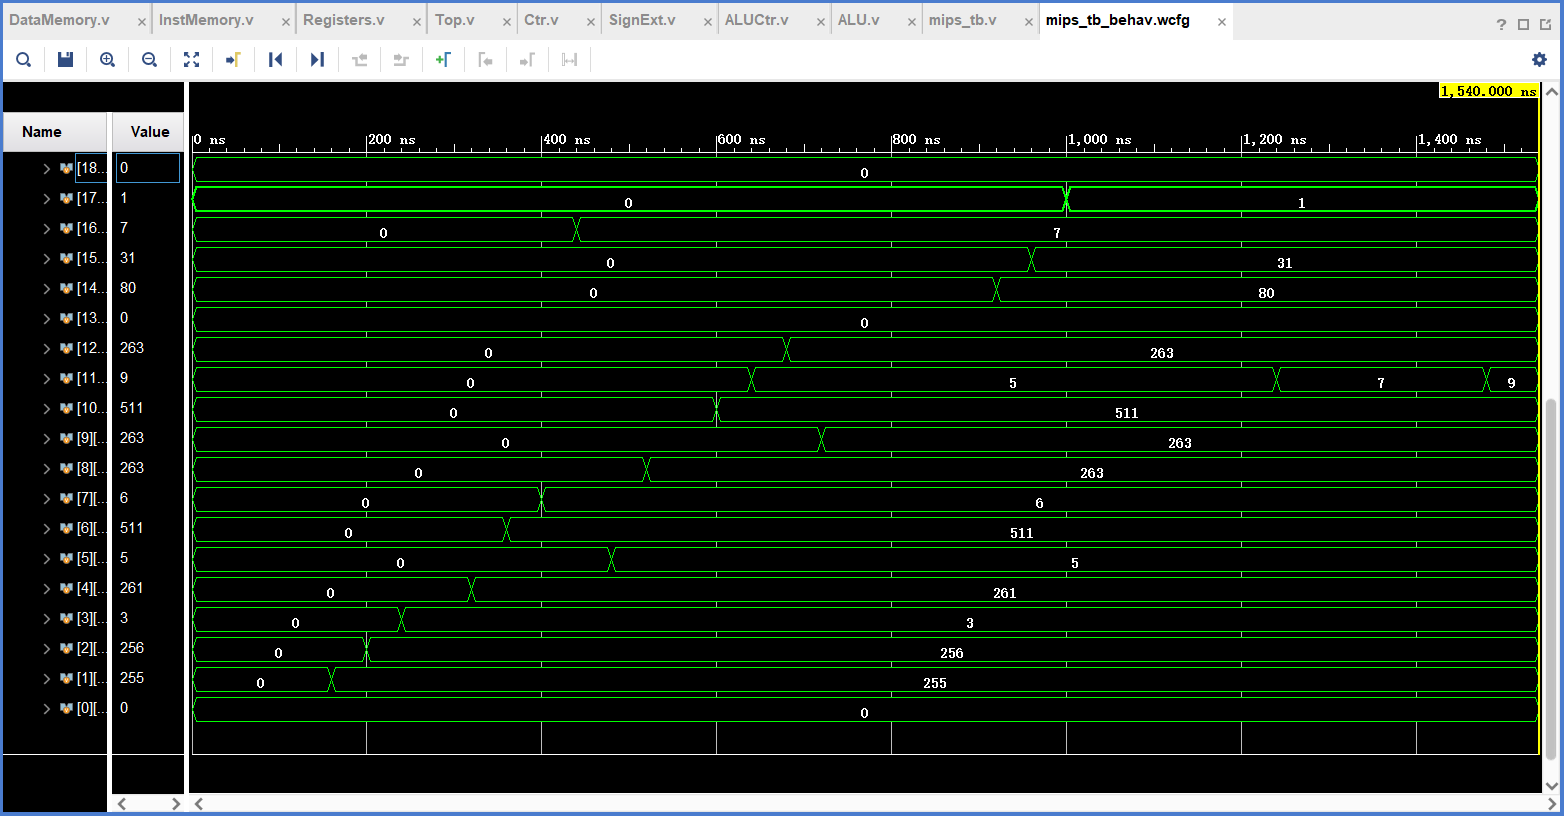
\includegraphics[width=7in]{1.png}
    \caption{MIPS多周期流水线处理器硬法测试结果}
    \label{fig1}
\end{figure}

对照图 \ref{fig1} 与表 \ref{tab3} 中的执行结果可知,运行结果完全正确,仿真成功,说明整个MIPS多周期流水线处理器实现正确。同时,我们可以将图 \ref{fig1} 与单周期MIPS处理器的测试图进行比较,也可以得出运行结果一致的结论。此外,在顶层模块中包含着许多注释,去掉部分注释可以在过程中输出相应的内容,通过这些内容可以验证指令执行的正确性,在这里就不详细展开。

接下来,我们进行\underline{软法测试(利用插入空指令的软件方法消除冒险)}。测试结果如图 \ref{fig2} 所示。

\begin{figure}[htbp]
    \centering
    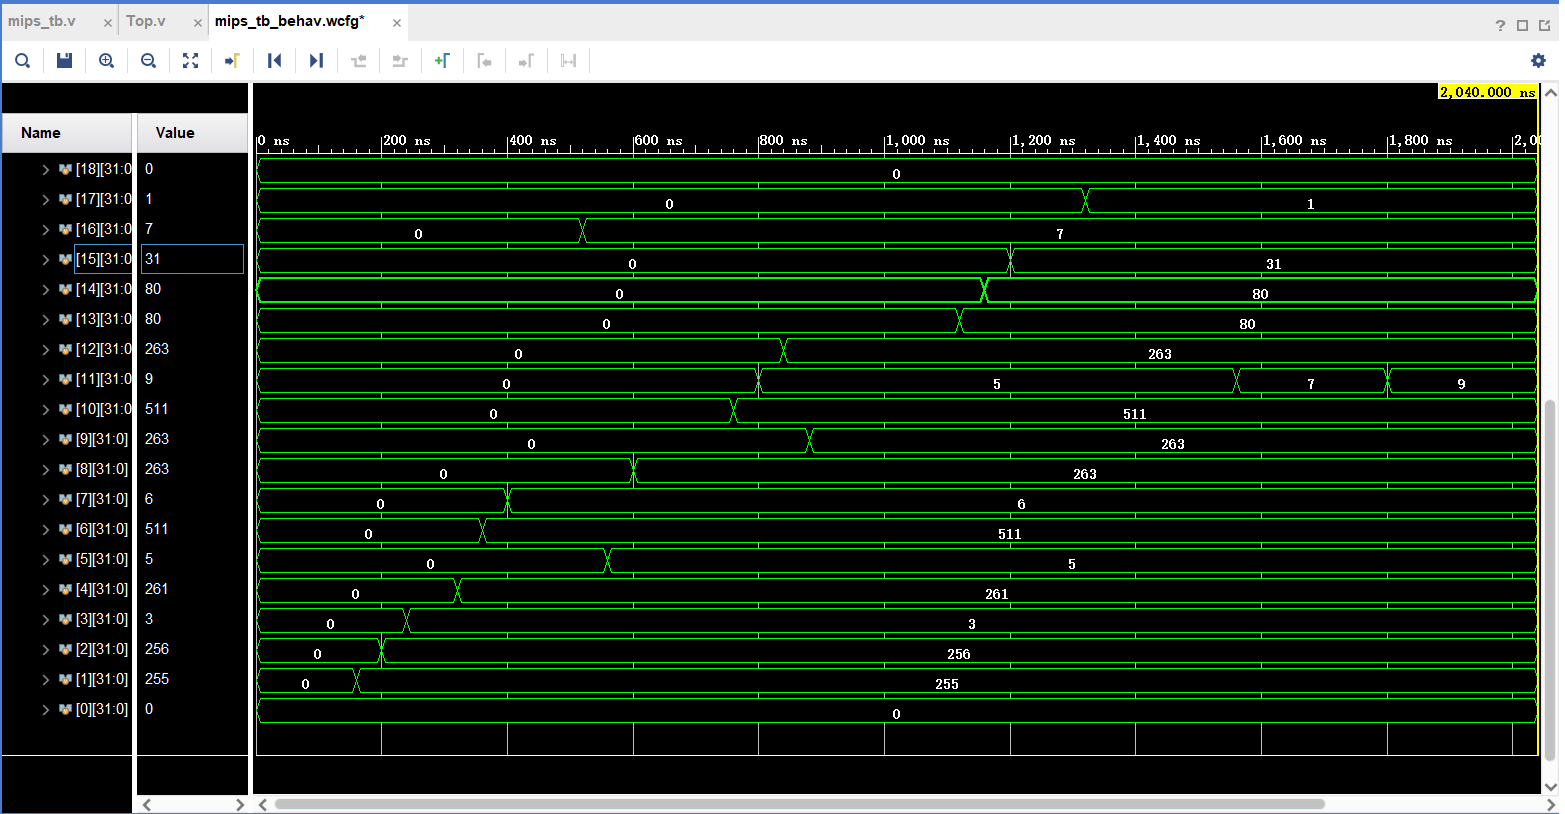
\includegraphics[width=7in]{2.png}
    \caption{MIPS多周期流水线处理器软法测试结果}
    \label{fig2}
\end{figure}

对比软硬方法仿真的结果,可以发现结果完全相同,只是软法仿真的运行速度较慢(由于插入了较多的空指令来消除冒险),这也侧面说明了我们设计的流水线处理器的硬件解决方案的高效性。

综上,经过详尽的测试,我们可以得出结论,我们的支持31指令的MIPS多周期流水线处理器实现正确。

\section{总结与反思}\label{section5}

本实验实现了一个完整的支持31指令的MIPS多周期流水线处理器,以实验三、四的模块以及实验五的单周期MIPS处理器为基础,对部分模块进行重新设计,添加了部分新的控制信号,并且较为完整地实现了流水线技术。通过这次实验,我加深了对于MIPS处理器的数据通路、信号通路等的了解,同时对于流水线有了更加深入的认识,充分理解了流水线中的段寄存器(segment registers)、前向通路(forwarding)、流水线停顿(stall)以及预测不转移(predict-not-taken)等技术的原理以及作用,而且通过代码实现了这些技术,令我收获颇丰。

同时,在调试的过程中,我对MIPS处理器的完整31指令也有了更加深刻的理解;通过自行编写对应的汇编代码、手动模拟汇编代码的运行结果、与自己写的处理器的运行结果进行对照等过程,对汇编代码也有了更加深刻的理解。同时,由于多周期处理器的调试过程中同时涉及多条指令,调试起来比较麻烦,总结调试的经验我认为,适当在代码中加入输出的指令有助于调试复杂、大型的代码,这种方法让我在调试流水线时省下了不少力气。

在结果验证中,我通过软硬方法的比对,将结果加以对比验证,得到了硬件方法效率更高的结论,这也让我更加深入理解了软件方法与硬件方法的优劣之处。

总之,我认为这次实验令我受益匪浅。


\section{致谢}\label{section6}
感谢本次实验中指导老师在课程微信群里为同学们答疑解惑;

感谢上海交通大学网络信息中心提供的远程桌面资源;

感谢计算机科学与工程系相关老师对于课程指导书的编写以及对于课程的设计,让我们可以更快更好地学习相关知识,掌握相关技能;

感谢电子信息与电气工程学院提供的优秀的课程资源。
%\bibliographystyle{plain}
%\bibliography{ref}

\clearpage
\begin{appendices}
\section{设计文件代码实现}\label{appsection1}
\subsection{各模块的代码实现}\label{appsection1.1}

\begin{itemize}
\item 主控制器(Ctr)参见代码文件 \texttt{Ctr.v}。
\item 算术逻辑运算单元(ALU)参见代码文件 \texttt{ALUCtr.v}。
\item 算术逻辑运算单元(ALU)参见代码文件 \texttt{ALU.v}。
\item 寄存器(Register)参见代码文件 \texttt{Registers.v}。
\item 存储器(Data Memory)参见代码文件 \texttt{DataMemory.v}。
\item 指令存储器(Instruction Memory)参见代码文件 \texttt{instMemory.v}。
\item 有符号扩展单元(Sign Extension)参见代码文件 \texttt{SignExt.v}。
\item 数据选择器(Mux)参见代码文件 \texttt{Mux5.v} 与 \texttt{Mux.v},分别表示5位与32位数据选择器。
\item 我们将程序计数器模块(PC)嵌入顶层模块(Top)中进行实现,因此没有单独的设计文件。
\end{itemize}
\subsection{顶层模块(Top)的代码实现}\label{appsection1.2}
参见代码文件 \texttt{Top.v}。
\section{激励文件代码实现}\label{appsection2}
参见代码文件 \texttt{mips\_tb.v}。
\end{appendices}

\end{document}
